\chapter{Visual C++}
\label{chap:Visual_C++}

Visual C++ is an IDE for writing C++ codes in Windows.
Windows provides 2 core library: CRT (Sect.\ref{sec:CRT})
and C++RT (Sect:\ref{sec:C++_RT}).

Visual C++ Express provides a subset functionality from other Visual C++
editions.

\section{Visual Studio versions}



\subsection{Visual C++ 2002, 2003}

It has \verb!Managed C++! (Sect.\ref{sec:managed_C++}).

It allows local variables defined inside loops to have scope outside the loop (\textcolor{red}{which is obsolete since VS 2005}).
\begin{verbatim}
for (int i=0; i<max; i++) { // do something } if (i>0) { // do something else }
\end{verbatim} 

Undeclared static variables (both global and local) has default type \verb!integer! (\textcolor{red}{which is obsolete since VS 2005})
\begin{verbatim}
const BUFLEN=255;  // which is understood as 'const int BUFFLEN=255;'
\end{verbatim}
Since VS 2005, you will get error
\begin{verbatim}
error C4430: missing type specifier - int assumed. Note: C++ does not support default-int
\end{verbatim}

\subsection{Visual C++ 2005}
\label{sec:VC++_2005}

Visual C++ 2005 has made major changes to Visual C++ libraries.
Several methods in Standard C++ Library (Sect.\ref{sec:CRT}) have been
identified as potentially unsafe (e.g. lead to buffer overrun or other code defect). Visual C++ 2005 comes
with the so-called Safe Libraries: these safer methods all end in \verb!_s!, and
prefix with an underscore \verb!_!.

Example: 
\begin{verbatim}
basic_string::copy              basic_string::_Copy_s
basic_stream::read              basic_stream::_Read_s
\end{verbatim}
\url{https://msdn.microsoft.com/en-us/library/vstudio/aa985872(v=vs.80).aspx}

\url{https://msdn.microsoft.com/en-us/magazine/cc163794.aspx}

Other changes:
\begin{itemize}
  \item local variable cannot be used outside the scope
  \item all variables need to have explicit type.
  \item new \verb!Safe C! and \verb!Safe C++! libraries
  
   These libraries provide more secure versions for many of the oldfangled C
   runtime (CRT) functions you know and love: strcpy, fopen and others.
   
   \item MFC: minor changes only
   \begin{itemize}
     \item \verb!CWnd::OnNcHitTest! return LRESULT (instead of UINT)
    \end{itemize}
\end{itemize}
\url{https://msdn.microsoft.com/en-us/magazine/cc163602.aspx}

We can also write GUI application using WinForms (check GUI Development ebook).


Managed C++ is replaced by C++/CLI (Sect.\ref{sec:C++/CLI}). 
Since VS 2005 and above, to allow compiling the deprecated Managed C++ (Sect.\ref{sec:managed_C++}), we need to use the compiler
option
\begin{verbatim}
/clr:oldSyntax
\end{verbatim}
This link describes how to port code from Managed C++ to C++/CLI:
\url{http://msdn.microsoft.com/en-US/library/b23b94s7(v=vs.80).aspx}

% C++/CLI includes
% new syntax for writing C++ application that can use managed code, i.e. code to
% run on CLR like any other .NET languages (C\#, VB.NET). You need to compile C++/CLI codes with
% \verb!/clr:[option]! compiling option.

% \begin{mdframed}
% \end{mdframed} 

% REMEMBER: The new syntax is not part of the ISO/ANSI C++ standard, but is a set
% of extension to C++, standardized in the name Ecma C++/CLI Standard.
% \url{http://msdn.microsoft.com/en-US/library/xey702bw(v=vs.80).aspx}





\subsection{Visual C++ 2008}
\label{sec:VS_2008}

VC++ 2008 has 3 main components:
\begin{enumerate}
  \item compiler tools: support native code (targetting x86, x64 and Itanium) or
  CLR (common language runtime)
  \item libraries: industry-standard ATL (active template library), MFC
  (microsoft foundation class) libraries + standard libraries (iostreams, STL
  (standard template library), CRT (C runtime library)). It also add 
  security-enhanced alternatives to functions that are known to pose security
  issues.
  
  It has STL/CLR library to bring STL to managed codes. 
  
  A Microsoft-specific library (C++ Support Library) with new features for data
  marshalling: to simplify codes targetting CLR.
  
  \item integrated development environment (IDE): supports project management,
  and configuration (better support for large projects), source-code
  editing/browsing/debugging. 
  
  IntelliSense can make informed, context-sensitive suggestions on the codes.
  
\end{enumerate}
Apart from conventional GUI application development, it also supports Web
application development: with smart-client Windows-based application,
thin-client and smart-client mobile devices.

To create a CUDA project
\begin{enumerate}
  \item Create new project: Other Languages - Visual C++ - ``Empty project''
  
  %(Other Project Types - Setup and Deployment -
  %Setup Wizard) Choose ``Windows application'',
   \item Create .c or .cpp files: to implement your host (serial) code 
   \item Create .cu files: to implement your wrappers and kernels
   \item Right-click on Projects, select ``Custom Build Rule''
   
   Choose the first one (NvCudaRuntimeApi.rules) if you have only one version of
   CUDA installed or you always want to use the latest one.
   \begin{verbatim}
   NvCudaRuntimeApi.rules 
   
   Cuda.rules
   
   NvCudaRuntimeApi.v3.2.rules
   (CUDA Driver API Build Rule (v3.2))
   
   NvCudaDriverApi.v3.2.rules
   (CUDA Runtime API Build Rule (v3.2))
   \end{verbatim}
  You can choose \verb!NvCudaRuntimeApi.v3.2.rules!. This means that instead
  of looking for the CUDA Toolkit in \verb!%CUDA_PATH%! it will look in
  \verb!%CUDA_PATH_V3_2%!, which in turn means that you can have multiple
  versions of the CUDA Toolkit installed on your system and different projects
  can target different version.
   
  \verb!Cuda.rules! is recommended to use in CUDA Toolkit 3.1 and earlier
  (provided by Nvidia with the SDK) that supports the latest compiler flags in a
  friendly manner. 
   
   \item Right-click Project Properties, then select
   \begin{verbatim}
Linker -> General   --> Additional Library Directories
    $(CUDA_PATH)\lib\$(PlatformName)
Linker -> Input  --> Additional Dependencies
   cudart.lib    
   \end{verbatim}
 Remember to do it for all building configurations.
 Also, similar to above setting, if you want to stabilise on a specific CUDA
 Toolkit version then you should replace \verb!CUDA_PATH! with \verb!CUDA_PATH_V3_2!.   
   
   \item (Optional) add CUDA include files to the search path (if the project
   has any .cpp files) by right-click Project Properties, select
 \begin{verbatim}
C/C++ --> General --> Additional Include Directories
    $(CUDA_PATH)\include	//if CUDA 3.2
    $(CUDA_INC_PATH)		//if CUDA 3.1
 \end{verbatim}
   
   \item Change the code generation to use statistically load C runtime to
   match CUDA runtime 
 \begin{verbatim}
C/C++ --> Code Generation --> Runtime Libraries	
    use /MT or /MD (depending on building the binary or library) for RELEASE
    use /MTd or /MDd (...) for DEBUG
   
 \end{verbatim}   
 Having mismatched version of the C runtime can cause a variety of problems; in
 particular if you have any errors regarding LIBCMT (e.g. LNK4098: defaultlib
 'LIBCMT' conflicts with use of other libs) or multiply defined symbols for
 standard library functions, then this should be your first suspect.  
 
 \item To enable syntax hightlighting:
 \begin{verbatim}
<sdk_install_dir>\C\doc\syntax_highlighting\visual_studio_8 
 \end{verbatim} 
 
 To enable Intellisense support, modify Windows registry (replace 9.0 with 8.0
 for VS2005 instead of VS2008)
 \begin{verbatim}
[HKEY_CURRENT_USER\Software\Microsoft\VisualStudio\9.0\Languages\Language Services\C/C++]
"NCB Default C/C++ Extensions"=".cpp;.cxx;.c;.cc;.h;.hh;.hxx;.hpp;.inl;.tlh;.tli;.cu;.cuh;.cl" 
 \end{verbatim}
 
 \item Avoid using Cutil if possible
 
 The reason is that this helper utilities do so many checking that may not be
 necessary if you know your code well enough. A lot of the cutil functionality
 is provided through online functions or macros, but some is provided by the
 static library cutil32D.lib (or 64, or without D for release mode). Make sure
 you have built cutil and are linking with the lib.  
\end{enumerate}


\url{http://stackoverflow.com/questions/2046228/how-do-i-start-a-new-cuda-project-in-visual-studio-2008}

%\subsection{manifest}

A default CRT/MFC application created using VS2008 need to use DLL-version of
CRT/MFC which are not pre-installed on any operating system. You need either
\begin{enumerate}
  \item Deploy CRT/MFC DLLs with your application
  (Sect.\ref{sec:deploy_CRT/MFC})
  \item Install \verb!vcredist_x86.exe/vcredist_x64.exe! 
  \item Statistically link CRT/MFC to the code when you compile.
\end{enumerate}


\subsubsection{Microsoft.VC90.CRT or Microsoft.VC90.MFC}
\label{sec:deploy_CRT/MFC}

When you deploy your application, written in Visual C++, you can copy either the
two folders
\begin{verbatim}
C:\Program Files (x86)\Microsoft Visual Studio 9.0\VC\redist\x86\Microsoft.VC90.CRT
C:\Program Files (x86)\Microsoft Visual Studio 9.0\VC\redist\x86\Microsoft.VC90.MFC
\end{verbatim}
into the same directory with your program. In the two folders above, each has
the following files
\begin{verbatim}
//folder 1
Microsoft.VC90.CRT.manifest
msvcr90.dll
msvcp90.dll
msvcm90.dll

//folder 2
Microsoft.VC90.MFC.manifest
mfc90.dll
mfc90u.dll
mfcm90.dll
mfcm90u.dll
\end{verbatim}

However, this won't work if you installed VS2008-SP1 (service pack 1). The
problem is that VS2008 SP1 overrites all the files in \verb!VC\redist! directory
with the new version. To resolve the problem on your compiled program, you
should update the content of either the file 
\verb!Microsoft.VC90.CRT.manifest! or \verb!Microsoft.VC90.MFC.manifest!. 

\url{http://blog.kalmbach-software.de/2009/05/27/deployment-of-vc2008-apps-without-installing-anything/}

\subsection{Visual Studo 2010}
\label{sec:VS2010}

When using VS 2010, you are required to convert your existing solutions/projects
to VS 2010 format. One major change is that VCBuild is replaced by MSBuild
(Sect.\ref{sec:MSBuild}). Also, you need to change your project's Target
Framework Version to .NET 4.0.

A custom build rules with \verb!.rules! file is replaced by a number of modules
that need to be specified to make a set of custom build rules to work.
The problem is that MS decided to change the old ".rules" syntax of VS2008 to
something even more messy in VS2010. VS2010 is supposed to convert the old
.rules file, but it doesn't work.

To be able to compile CUDA 3.2 code in Visual Studio 2010, we still need to have
either (1) Visual Studio 2008, (2) VC9 C compiler.  This is the next steps:
\begin{enumerate}
  \item  Setup
VC9INSTALLDIR environment variable to point to VS C++ 2008 installation directory
\begin{verbatim}
C:\Program Files\Microsoft Visual Studio 9.0\VC\
\end{verbatim}
 Make sure the trailing "\" is added to the path.
  
  \item attach a zip file contains 3 files for .cu build rules
  (cuda-build-rules.zip)
  
  The rule files here are slightly different from that in the link
  \url{http://social.msdn.microsoft.com/Forums/en/vcprerelease/thread/d24cba9c-ec87-4e27-83c2-1343a2e62a40}
. There was a problem where double quotes needed to be added in the cuda.props
file, since Windows allows spaces in paths.
  
\url{https://devtalk.nvidia.com/cmd/default/download-comment-attachment/42196/}
  
  Unpack and copy to
\begin{verbatim}
C:\Program Files (x86)\MSBuild\Microsoft.Cpp\v4.0\BuildCustomizations
\end{verbatim}
This path depends on where you installed MSVC2010.


  \item  Open MVSC2010, and convert or create a new project
  
  
  \item Go to menu item "Project | Build Customizations..." and make sure to
  select the "cuda(.targets, .props)" rule.
  
  \item Setup your options for .cu file in the project
\end{enumerate} 
If it still gives you errors the "-1" errors, go to the output window in MSVC
and copy the command it's trying to execute, and see what it's doing. 

Caveats: You should be able to compile .cpp files with the VC10 compiler, .cu
files with \verb!nvcc! (VC9), and link with the runtime in VC10--works for me. However,
you may get problems with linking in some situations, e.g.,
\begin{verbatim}
unresolved external symbol "public: static void __cdecl
std::_String_base::_Xran(void)" (?_Xran@_String_base@std@@SAXXZ)
\end{verbatim}

In that case, you may have to rip apart the .cu file so that
it only has kernel code, device code, and kernel calls, so that it doesn't use
the C runtime. 




\subsection{Visual Studio 2012}

To update project to VS 2012:
\url{http://msdn.microsoft.com/en-us/library/hh266747(v=vs.110).aspx}



\subsection{Visual Studio 2013}


New:
\begin{enumerate}
  \item .NET Framework 4.5.1
\end{enumerate}

Update:
\begin{enumerate}
  \item Update 4:
  \url{http://www.microsoft.com/en-us/download/details.aspx?id=44921}
\end{enumerate}

\subsection{Visual Studio Community 2013}

Visual Studio Community 2013 is a new free edition of Visual Studio that
provides easy access to the Visual Studio core toolset. 

This is a new, full-featured version of Visual Studio 2013 that will be
available at no cost to independent developers, students, small companies and
others not making enterprise applications.  In particular, an unlimited number
of users within an organization can use Visual Studio Community for the
following scenarios: in a classroom learning environment, for academic research,
or for contributing to open source projects; and for all other usage scenarios:
in non-enterprise organizations, up to 5 users can use Visual Studio Community.

\url{http://www.visualstudio.com/products/visual-studio-community-vs}


\subsection{Visual Studio 2015}

Visual Studio 2015 and .NET 2015 with new features for building applications
that run on platforms including Windows, Linux, iOS and Android.

To further support cross-platform mobile development with .NET, as part of their
strategic partnership, Microsoft and Xamarin announced a new streamlined
experience for installing Xamarin from Visual Studio, as well as announced the
addition of Visual Studio support to its free offering Xamarin Starter Edition -
available later in the year. In addition, for Web developers interested in
building cloud-powered apps that target mobile devices, Microsoft delivered the
final release of Apache Cordova tools.

\url{http://www.microsoft.com/en-us/download/confirmation.aspx?id=44934}

\subsection{Visual Studio Online}

It is an online service for development projects, by announcing additional
capabilities for the service, including these:
\begin{enumerate}
  \item Release Management as a service: 
   to enable customers to automate and manage application releases without the
   need to set up or maintain any service infrastructure.
  
  \item Cloud Deployment Projects:  to allow organizations to more easily and
  reliably provision and configure development, test and production environments
  in Azure. 
\end{enumerate}


\subsection{VCBuild to MSBuild}

There is a major change in the buildtool for Visual C++ since VS 2010 which
switched from VCBuild (Sect.\ref{sec:VCBuild}) to MSBuild
(Sect.\ref{sec:MSBuild}).
There are two tools to help updating your projects
\begin{enumerate}
  \item a single project solution: 
  
\begin{verbatim}
vcupgrade.exe <filename>.vcproj
\end{verbatim}  

  \item multiple-project solution: use devenv to converts the whole solutions
  (.sln) and all of the projects within.  Once the project or solution has been
  converted without errors, you can use MSBuild 
\begin{verbatim}

C:\Program Files (x86)\Microsoft Visual Studio 12.0\Common7\IDE\
devenv [SolutionFile | ProjectFile] /upgrade

devenv "MYProject.sln" /upgrade
\end{verbatim}
The whole solution is automatically backed into a \verb!Backup! newly created
folder in the current directoy. 

Troubleshooting when the conversion is not successfull: use a text editor to
open the project file and scan for incorrect file path (especially those
contains Visual Studio version number) and fix it.
\url{http://msdn.microsoft.com/en-us/library/ms185327.aspx}



\end{enumerate}

\subsection{Change TargetFrameWorkVersion}

Modifying this is not supported in VS Express 2012.

The target .NET framework version is given in (.vcxproj) file,
a XML-based file 
\begin{verbatim}
<TargetFrameworkVersion>v4.0</TargetFrameworkVersion>
\end{verbatim}
and, since VS 2013, it is replaced by \verb!ToolsVersion! attribute in the
\verb!Project! element.
\begin{verbatim}
<Project DefaultTargets="Build" ToolsVersion="4.0" xmlns="http://schemas.microsoft.com/developer/msbuild/2003">
\end{verbatim}

The value here appears on 
\begin{verbatim}
Solution Explorer --> Project's Properties -->
       Properties Page: expand Common Properties, select
             Framework and References.
\end{verbatim}



\subsection{Change TargetPlatformToolset}
\label{sec:change-MSBuild-toolset-version}

Modifying this is not supported in VS Express 2012.

Change MSBuild target platform toolset, Fig.\ref{fig:MSBuild_platform-toolset}

\begin{verbatim}
Project's Property Page: expand Configuration Properties
   --> select General, on right pane
   --> select Platform Toolset
\end{verbatim}
%\section{VCBuild to MSBuild }

\section{History of Build tools}
\label{sec:history_Build-tools}

This section discusses tools to help automate build the source-code at the
project level. To know about tools that help managing
installing/removing/upgrading packages (i.e. compiled code), then we need to
read the book {\bf Project Management}, Chapter {\it Package Manager}.

Now, return to the topic of this section. In order to help automating the
building process of a project contains many files, several build tools have been
developed. One of the first and widely used in Unix/Linux world is UNIX's {\bf
Make}. A Java successor of Make is {\bf Apache Ant} which use XML-based
configuration file.

Microsoft .NET remake of Apache Ant and open-source is called {\bf NAnt}
(Sect.\ref{sec:NAnt}). Then, Microsoft used VCBuild (Sect.\ref{sec:VCBuild}),
before switching to MSBuild (Sect.\ref{sec:MSBuild}). The binary file is \verb!MSBuild.exe!. 
NAnt has more features out of the box, but MSBuild has a much better fundamental
structure (item metadata rocks) which makes it much easier to build reusable
MSBuild scripts. 

MSBuild run on Visual Studo (.sln) file, and generate (.proj) files. 
\begin{itemize}
  \item C\# project (.csproj) file which is acutally a (.proj) file with
  importing Microsoft.CSharp.targets
  
  \item C++ project (.vcxproj) file (Visual Studio 2013+) 
\end{itemize}
MSBuild was
first part of .NET framework.

TFSBuild (Team Foundation Build) started with Visual Studio 2005 and is
designed for build manager at enterprise level. It is based on MSBuild 3.5. It
is an extensible system that can automate processes (1) synchronize the sources,
(2) compile the code, (3) run unit tests, (4) perform code analysis, (5) release
build on a file server, (6) publish build reports, etc. It works with
\begin{itemize}
  \item Team Foundation Version Control
  \item Team Foundation Server
\end{itemize}

% enable you to specify the build computer to use, the solution to build, the drop location, the test to run, etc.

Books:
\url{http://www.amazon.com/Inside-Microsoft-Build-Engine-Foundation/dp/0735645248}

\url{http://www.zvolkov.com/clog/2009/04/12/catching-up-on-msbuild/}

\section{VCBuild}
\label{sec:VCBuild}

You are recommended to read Sect.\ref{sec:history_Build-tools} first.

VCBuild is a command-line build tool \verb!vcbuild.exe! being used in Visual
Studio 2008 and earlier.
\begin{verbatim}
C:\Program Files (x86)\Microsoft Visual Studio 9.0\VC\vcpackages\vcbuild.exe
\end{verbatim}

Since Visual Studio 2010, VCBuild is replaced by MSBuild
(Sect.\ref{sec:MSBuild}). Along with that, the project extension
(\verb!.vcproj!) in VCBuild is replaced by \verb!.vcxproj! in MSBuild.
\url{http://msdn.microsoft.com/en-us/library/ee862524.aspx}

\section{MSBuild}
\label{sec:MSBuild}

You are recommended to read Sect.\ref{sec:history_Build-tools} first.

MSBuild is the replacement for VCBuild (Sect.\ref{sec:VCBuild}) since Visual
Studo 2010 (Sect.\ref{sec:VS2010}). Along with that, there are some changes
to certain file types. The new VC++ project file format is \verb!.vcxproj!
extension, rather than \verb!.vcproj!.

\begin{mdframed}
The major difference is that VCBuild builds all Configuration and Platform
matrix by default; while MSBuild only built Debug|Win32 by default.
In MSBuild, any feature enabled by using \verb!/p[property]! can also be enabled
by setting the environment variable with the respective name
\end{mdframed}


MSBuild Toolset contains a number of files
\begin{itemize}
  \item microsoft.common.targets: defines steps in the standard build process
  for .NET projects (Visual Basic, Visual C\#)
  \item microsoft.common.tasks: 
  \item compilers (such as csc.exe, vbc.exe)
\end{itemize}
They are XML-based files and should not be modified. MSBuild 2.0 toolset can be
used to compile code for .NET framework 2.0 only; while newer versions can be
used to compile code to more than one versions of .NET frameworks.

The version of the MSBuild Tool being used is defined in
\verb!MSBuildToolVersion! predefined properties, which can be changed using the
Project Properties dialog box (Sect.\ref{sec:change-MSBuild-toolset-version}).

\begin{figure}[hbt]
  \centerline{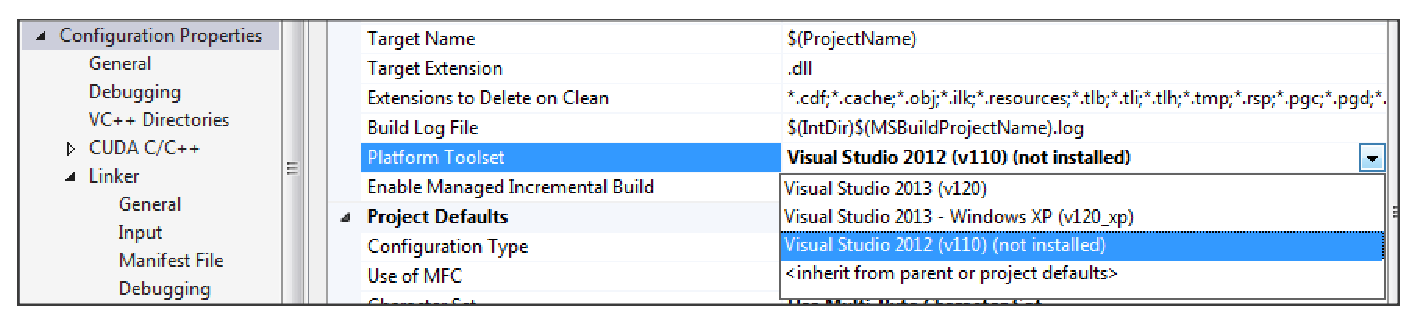
\includegraphics[height=2.7cm,
    angle=0]{./images/MSBuild_platform-toolset.eps}}
\caption{MSBuild platform toolset}
\label{fig:MSBuild_platform-toolset}
\end{figure}


\subsection{Predefined Properties}

MSBuild uses a set of predefined properties (macros) to store information about
the project file and the MSBuild binaries.
\footnote{\url{http://msdn.microsoft.com/en-us/library/ms164309.aspx}}
\begin{verbatim}

MSBuildThisFileFullPath            return the fullpath to the current (.targets)
                                   file, e.g. CUDA 6.0.targets
MSBuildThisFileExtension

MSBuildThisFileName

MSBuildToolsPath				  (cannot be overridden) the installation path of the
                                  MSBuild version that is associated with the
                                  value being chosen in MSBuildToolsVersion
      32-bit MSBuild 12.0+ : %ProgramFiles%\MSBuild\12.0\bin
      64-bit MSBuild 12.0+ : %ProgramFiles%\MSBuild\12.0\bin\amd64 
                                  
MSBuildToolsVersion                                                 
\end{verbatim}

\subsection{.props (property sheet)}

There are multiple property groups (import groups) instead of one. This allows
the last definition overrides the preceding ones.

\begin{verbatim}
<Import Project="$(VCTargetsPath)\Microsoft.Cpp.Default.props" />

<Import Project="$(VCTargetsPath)\Microsoft.Cpp.props" />

 <ImportGroup Label="ExtensionSettings">
    <Import Project="CUDA 6.0.props" />
  </ImportGroup>
  
  <ImportGroup Condition="'$(Configuration)|$(Platform)'=='Release|x64'" Label="PropertySheets">
    <Import Project="$(UserRootDir)\Microsoft.Cpp.$(Platform).user.props" Condition="exists('$(UserRootDir)\Microsoft.Cpp.$(Platform).user.props')" Label="LocalAppDataPlatform" />
  </ImportGroup>  
\end{verbatim}

\begin{enumerate}
  \item Default settings for a VC++ Project (not tool-specific), i.e.
  definitions for properties like Platform, PlatformToolset, OutputPath, TargetName, UseOfAtl,
  etc.
\begin{verbatim}
Import Project="$(VCTargetsPath)\Microsoft.Cpp.default.props" />
\end{verbatim}  

  \item Default values for many tool-specific properties, e.g. compiler's
  Optimization, WarningLevel properties, Midl tool's TypeLibraryName property,
  etc.
\begin{verbatim}
<Import Project="$(VCTargetsPath)\Microsoft.Cpp.props" />
\end{verbatim}
\end{enumerate}


Example:
\begin{verbatim}
<Project DefaultTargets="Build" ToolsVersion="4.0" xmlns='http://schemas.microsoft.com/developer/msbuild/2003' >
  <ItemGroup Label="ProjectConfigurations" />
  <PropertyGroup Label="Globals" />
  <Import Project="$(VCTargetsPath)\Microsoft.Cpp.default.props" />
  <PropertyGroup Label="Configuration" />
  <Import Project="$(VCTargetsPath)\Microsoft.Cpp.props" />
  <ImportGroup Label="ExtensionSettings" />
  <ImportGroup Label="PropertySheets" />
  <PropertyGroup Label="UserMacros" />
  <PropertyGroup />
  <ItemDefinitionGroup />
  <ItemGroup />
  <Import Project="$(VCTargetsPath)\Microsoft.Cpp.targets" />
  <ImportGroup Label="ExtensionTargets" />
</Project>
\end{verbatim}

\url{http://blogs.msdn.com/b/visualstudio/archive/2010/05/14/a-guide-to-vcxproj-and-props-file-structure.aspx}

\subsection{.targets}

There can be one or more \verb!.targets! files in your project. Each file
contains items, properties, targets, and tasks for common scenarios. These files
are typically automatically imported from somewhere else
\begin{itemize}
  \item Microsoft.CSharp.targets
  \item Microsoft.Common.targets
  \item Microsoft.VisualBasic.targets
  \item CUDA 6.0.targets
  \item CUDA 6.5.targets
\end{itemize}
Depending on the value of \verb!ToolsVersion!, the location is a subfolder of
\begin{verbatim}
<WindowsInstallationPath>\Microsoft.NET\Framework
\end{verbatim}
Example: ToolsVersion=4.0, then 
\begin{verbatim}
C:\Windows\Microsoft.NET\Framework\v4.0.30319
\end{verbatim}
The location of these file is defined in \verb!$(MSBuildToolsPath)!

If your project import one of these files, you will see this line in the Project
XML-based file
\begin{verbatim}
<Import Project="Microsoft.Common.targets" />
<Import Project="$(MSBuildToolsPath)\Microsoft.CSharp.targets" />
<Import Project="$(MSBuildToolsPath)\Microsoft.VisualBasic.targets" />
\end{verbatim}



\begin{verbatim}
http://msdn.microsoft.com/en-us/library/ms164312.aspx
\end{verbatim}

\subsection{MSBuild 4.5}

In VS 2012, MSBuild version number is 4.5 with .NET framework 4.5. 

You can build app targets to 
\begin{itemize}
  \item ARM processor
  \item
  \url{http://msdn.microsoft.com/en-us/library/hh162058(v=vs.110).aspx}
\end{itemize}


\subsection{MSBuild 12.0}

Since Visual Studio 2013, MSBuild is part of Visual Studio,
rather than .NET framework (4.5.1), and thus is installed under
\begin{verbatim}
C:\Program Files\MSBuild\.
\end{verbatim}
Also, the version number jumps to (version 12.0).


\url{http://msdn.microsoft.com/en-us/library/hh162058(v=vs.121).aspx}



\subsection{Build CUDA code in VS}

When adding CUDA acceleration to existing applications, the relevant Visual
Studio project files must be updated to include CUDA build customizations.
If you create a new project, remember to select
\begin{verbatim}
File-> New | Project... NVIDIA-> CUDA->
\end{verbatim}
and finally select a template for CUDA toolkit version, e.g. CUDA 6.5. runtime
template.  The new project is technically a C++ project (.vcxproj) that is
preconfigured to use NVIDIA's Build Customizations. 
So, all standard capabilities of Visual Studio C++ projects will be available.
If the location of CUDA toolkit is not standard, then under {\bf CUDA C/C++},
select {\bf Common}, select {\bf CUDA Toolkit Custom Dir}, and type the location
of the CUDA toolkit (you can use \verb!$(CUDA_PATH)! to use the latest
CUDA toolkit version).

If you have an existing project/solution and you want to add CUDA code.
To build CUDA code in Visual Studio, we need to define Custom Build Rules (or
Build Customization), which has already been defined by NVidia, you just need to
tell where the files are
\begin{enumerate}
  \item There are some additional settings you need to do, if you don't
  have Nvidia Nsight. From your project, select Custom Build Rules, select Find
  Existing. Browser to
\begin{verbatim}
C:\Program Files\NVIDIA Corporation\NVIDIA GPU Computing SDK\C
\end{verbatim}
and select CUDA.rules. This add two files (.targets and .props)

   \item Go to Project / Custom Build Rule (later changed to {\bf Build
   Customization}), and select the right CUDA toolkit version
   \footnote{\url{http://blogs.msdn.com/b/visualstudio/archive/2010/04/26/custom-build-steps-tools-and-events.aspx}}
\begin{verbatim}
``Enable CUDA rule''

CUDA 3.1 (.targets, .props)
CUDA 3.2 (.targets, .props)
CUDA 6.0 (.targets, .props)
CUDA 6.5 (.targets, .props)
\end{verbatim}
\url{http://blog.cuvilib.com/2011/02/24/how-to-run-cuda-in-visual-studio-2010/}

   \item You can also configure to use the latest version of CUDA toolkit
   (whose path is given in \verb!$(CUDA_PATH)! environment variable), by opening
   the Project's Properties page, Under CUDA C/C++, select Common, and set the
   CUDA Toolkit Custom Dir field.
\end{enumerate}

Select Include files:
\begin{itemize}
  \item Click Tools / Options / Project and Solutions / VC++ Directories
  \item Specify Include, then show the Directories
  \item For each line below, click 'New' and add them 
\begin{verbatim}
C:\Program Files\NVIDIA Corporation\CUDA\include

C:\Program Files\NVIDIA Corporation\NVIDIA GPU Computing SDK\C\common\inc
\end{verbatim}
\end{itemize} 


Select Lib files
\begin{itemize}
  \item Do the same, sepecify Lib
\begin{verbatim}
C:\Program Files\NVIDIA Corporation\NVIDIA GPU Computing SDK\C\common\lib

C:\Program Files\NVIDIA Corporation\CUDA\lib64
\end{verbatim}  
\end{itemize}

Select the executable files
\begin{itemize}
  \item Do the same, specify the executables
\begin{verbatim}
C:\Program Files\NVIDIA Corporation\CUDA\bin64
\end{verbatim}
\end{itemize}


Select the Linker options
\begin{verbatim}
Project -> Properties  -> Linker -> Input
 -> Additional Dependencies
\end{verbatim}
add 
\begin{verbatim}
cudart.lib
cutil64D.lib
\end{verbatim}
then
\begin{verbatim}
Project -> Properties  -> Linker -> General

and add path
C:\Program Files\NVIDIA Corporation\NVIDIA GPU Computing SDK\C\common\lib

C:\Program Files\NVIDIA Corporation\CUDA\lib64
\end{verbatim}

Increase the stack Reserve size
\begin{verbatim}
Project -> Properties ->
     Linker -> System -> Stack Reserve Size=500000000
\end{verbatim}

Now you can add your CUDA (.cu) source code. 

The last step is to specify the location where to put the output file (which
can be executable file or dynamic-link library DLL). Here, we use Project's
Property page $\rightarrow$ Linker, and modify \verb!Output File! textbox


In order to debug the CUDA code, you need to copy necessary CUDA library files
to the \verb!$(Outdir)! folder where the binary file is created. You can do this
by using Post-Build Event (Sect.\ref{sec:MSBuild_Events})
\begin{verbatim}
copy "$(CudaToolkitBinDir)\cudart*.dll" "$(OutDir)"
copy "$(CudaToolkitBinDir)\curand*.dll" "$(OutDir)"
\end{verbatim}
or you can get the error
\begin{verbatim}
The program can't start because cudart32_50_35.dll is missing from your
computer.
\end{verbatim}




\subsection{Build CUDA source code examples}

CUDA examples are stored in
\begin{verbatim}
%% Windows XP
C:\Documents and Settings\All Users\Application Data\NVIDIA Corporation\CUDA
Samples\v6.5

%% (newer)
C:\ProgramData\NVIDIA Corporation\CUDA Samples\v6.5
\end{verbatim}
\verb!C:\ProgramData! is a hidden folder.

Open the solution files from
\begin{verbatim}
C:\ProgramData\NVIDIA Corporation\CUDA Samples\v6.5\<category>\<sample_name>
\end{verbatim}
or the global solution files
\begin{verbatim}
C:\ProgramData\NVIDIA Corporation\CUDA Samples\v6.5
\end{verbatim}

From CUDA 6.x, CUDA samples are organized in categories
\begin{verbatim}
0_Simple
1_Utilities
2_Graphics
3_Imaging
4_Finance
5_Simulations
6_Advanced
7_CUDALibraries
\end{verbatim}

The environment variables are set automatically using the Buidl Customization 
\begin{verbatim}
CUDA 6.5.props
\end{verbatim}
which is installed as part of CUDA 6.5 toolkit. Location of this file

\begin{verbatim}
%% VS 2010
C:\Program Files (x86)\MSBuild\Microsoft.Cpp\v4.0\V100\BuildCustomizations

%% VS 2012
C:\Program Files (x86)\MSBuild\Microsoft.Cpp\v4.0\V110\BuildCustomizations

%% VS 2013
C:\Program Files (x86)\MSBuild\Microsoft.Cpp\v4.0\V120\BuildCustomizations
\end{verbatim}

The sample projects also use \verb!$(CUDA_PATH)! to detect the necessary files.

\subsection{Build CUDA code with a different CUDA toolkit version without
changing the Project's files}

In the command line, switch to the project's folder, and run
\begin{verbatim}
msbuild <projectname.extension> /t:Rebuild
    /p:CudaToolkitDir="drive:/path/to/new/toolkit/"
\end{verbatim}


\url{http://docs.nvidia.com/cuda/cuda-getting-started-guide-for-microsoft-windows/index.html#axzz3Fd0ryRW3}



\subsection{Build to 64-bit}

Solution / Configuration Manager / Active Solution Platform = New; select
\verb!x64! and import settings from win32.

Make sure Project / Properties / Linker / Advanced / Target Machine = x64

\subsection{Build a DLL}

You may need a module-definition (.def) file which 
 provide the linker with information about exports, attributes, and other
information about the program to be linked.

\begin{verbatim}
Project's Property
   --> LInker
      --> Input
          --> Module Definition File 
                    CUDAFluxEngine.def
\end{verbatim}

In that file, we specify which APIs are exported to use, or we can do explicitly
inside the code with
\begin{verbatim}
__declspec(dllexport) 
\end{verbatim}
as a way to specify exported functions.

\url{http://msdn.microsoft.com/en-us/library/28d6s79h.aspx}

\subsection{Build Events}
\label{sec:MSBuild_Events}

You can specify what to do before or after the build using
\begin{verbatim}
Project's Property
   --> Build Events
       --> Pre-Build Event
           Pre-Link Event
           Post-Build Event
\end{verbatim}

These are indeed batch files. The utility \verb!COMMAND.COM! read one line
from the batch file, execute command, and repeat the process (reading next
line from the file, execute that line). This applies to comment line as well,
i.e. each comment line causes one extra re-read of the batch file. To indicate
a comment line, it use REM (REMarks) to start a comment line.
\url{http://www.robvanderwoude.com/comments.php}

To put the comments or temporarily comment out a command, we put \verb!REM! in
the front
\begin{verbatim}
REM signtool sign /a $(TargetPath) xcopy /Y "$(TargetPath)" "C:\Deploy\$(TargetFileName)"
\end{verbatim}
\url{http://stackoverflow.com/questions/5626166/proper-way-to-put-comments-in-build-events-command-line}

\subsection{Build Linker}

Here, you specify where to put the output file which can be an executable file
or a dynamic-link library.

Make sure that
\begin{verbatim}
$(OutDir), $(TargetName) and $(TargetExt) 
\end{verbatim}
property values match the value specified in \verb!%(Link.OutputFile)!.

To specify additional dependencies, use
\begin{verbatim}
Project's Property
   --> LInker
      --> Input
        --> Additional Dependencies
                  ann.lib;nvapi64.lib;cudart.lib;curand.lib;
\end{verbatim}

\url{http://msdn.microsoft.com/en-us/library/y0zzbyt4.aspx}

NOTE:
\begin{verbatim}
/LTCG specified but no code generation required; remove /LTCG from the link
command line to improve linker performance
\end{verbatim}


\subsection{Build some projects in a solution}	


You can do this from the command-line
\begin{verbatim}
msbuild /P:Configuration=Release PACKAGE.vcxproj
\end{verbatim}
or using Visual Studio: right-click on Solution page, and select {\bf
Configuration Manager}.

You may get the error
\begin{verbatim}
warning MSB3270: There was a mismatch between the processor architecture of the
project being built "MSIL" and the processor architecture of the reference "DocumentServiceModel", "x86".
\end{verbatim}
if some projects in the same solution has a conflict built target between them.

If your solution have multiple projects and some of them are just libraries;
then if you select to debug, you may get the error
\begin{verbatim}
A project with an Output type of Class Library cannot be started directly
\end{verbatim}
To fix this, right click Solution's Property page
\begin{verbatim}
--> Common Properties --> Startup Project
\end{verbatim}
you can choose either below, but just to make sure the project you run is not
the one compiled into the library
\begin{itemize}
  \item Current selection
  \item Single startup project
  \item Multiple startup projects
\end{itemize}

\section{NAnt}
\label{sec:NAnt}

NAnt is used to automate builds.
NAnt 0.92 only supports .NET 4.0

\section{CUDA in Windows}

In order to program CUDA in Windows, you need
\begin{enumerate}
  \item CUDA-capable GPU
  \item a supported version of Windows
  \item a supported version of IDE, e.g. Visual Studio
  \item NVIDIA CUDA Toolkit (which include the driver as well)
  
Example: command line in silent mode  
\begin{verbatim}
<PackageName>.exe -s CUDAToolkit_6.5 Display.Driver
\end{verbatim}  
\end{enumerate}


The default installation location is
\begin{verbatim}

%% Toolkit
C:\Program Files\NVIDIA GPU Computing Toolkit\CUDA\v6.0

C:\Program Files\NVIDIA GPU Computing Toolkit\CUDA\v6.5


%% Samples  (hidden folder)
C:\ProgramData\NVIDIA Corporation\CUDA Samples\v6.0


%% Documentation

\end{verbatim}

There are two driver model can be used on Windows 7 and later
\begin{enumerate}
  \item WDDM: used for display devices
  \item Windows WDM: available for non-display device and Nvidia driver mode TCC
  (Tesla Compute Cluster) uses this. This is not supported in GeForce family.
  Advantages:
  \begin{itemize}
    \item use CUDA with Windows Remote Desktop
    \item use CUDA within processes running as Windows Services
    \item reduce latency in CUDA kernel launches + eliminate timeouts that can
    occur when running under WDDM due to Windows TDR
    \footnote{\url{http://msdn.microsoft.com/en-us/library/windows/hardware/ff570087(v=vs.85).aspx}}
  \end{itemize}
\end{enumerate}
TCC is enabled by default on most recent GPUs (and condition: it must not be
used for display), we can check with
\begin{verbatim}
nvidia-smi
\end{verbatim}

\subsection{Syntax hightlighting}


Visual Studio / Tools / Options / text Editor / File Extension.
\begin{verbatim}
Tools | Options | Projects | VC++ Build | C/C++ File Extensions (VS.NET)

Tools | Options | Projects and Solutions | VC++ Project Settings | C/C++ File Extensions (VS2005, VS2008)

Tools | Options | Projects and Solutions | VC++ Project Settings | Extensions To Include (VS2010)
\end{verbatim}

Then add \verb!cu!, \verb!cuh! to Microsoft Visual C++.
\url{http://stackoverflow.com/questions/14827160/how-do-i-enable-syntax-highlighting-of-cuda-cu-files-in-visual-studio-2010}

If you use Visual Studio 2012 or older, please continue the below steps.
To avoid syntax highlighting of CUDA keywords (like threadldx.x), we need to
include in the CUDA code (so that IDE won't show false syntax errors)
\begin{verbatim}
#include<device_launch_parameters.h>
\end{verbatim}
However, using this may cause \verb!nvcc!'s intrinsic compiler functions for arithmetic
to appear undefined if you have both
\begin{verbatim}
#include "cuda_runtime.h"
#include "device_launch_parameters.h"
\end{verbatim}
The fix is to remove those two includes from the project when you want to
compile.
\url{http://stackoverflow.com/questions/13966469/why-dont-the-cuda-compiler-intrinsics-fadd-rd-etc-work-for-me}

You may use \verb!usertype.dat! in (until CUDA 5.0)
\begin{verbatim}
C:\ProgramData\NVIDIA Corporation\CUDA
Samples\v5.0\doc\syntax_highlighting\visual_studio_8
\end{verbatim}
copy the content and append to the same file name (if existing) or copy (if the
file is not in the below folder) in the below folder
\begin{verbatim}

%% VS 2012 is being used
C:\Program Files\Microsoft Visual Studio 12.0\Common7\IDE
\end{verbatim}

Finally, restart the Visual studio

NOTE: Example of the usertype.dat file content
\begin{verbatim}
__global__
__host__
__device__
__constant__
__shared__
gridDim
blockIdx
blockDim
threadIdx
int1
uint1
int2
uint2
int3
uint3
int4
uint4
float1
float2
float3
float4
char1
char2
char3
char4
uchar1
uchar2
uchar3
uchar4
short1
short2
short3
short4
dim1
dim2
dim3
dim4
tex1D
tex1Dfetch
tex2D
__float_as_int
__int_as_float
__float2int_rn
__float2int_rz
__float2int_ru
__float2int_rd
__float2uint_rn
__float2uint_rz
__float2uint_ru
__float2uint_rd
__int2float_rn
__int2float_rz
__int2float_ru
__int2float_rd
__uint2float_rn
__uint2float_rz
__uint2float_ru
__uint2float_rd
__fadd_rz
__fmul_rz
__fdividef
__mul24
__umul24
__mulhi
__umulhi
__mul64hi
__umul64hi
min
umin
fminf
fmin
max
umax
fmaxf
fmax
abs
fabsf
fabs
sqrtf
sqrt
sinf
__sinf
sin
cosf
__cosf
cos
sincosf
__sincosf
expf
__expf
exp
logf
__logf
log
__syncthreads
\end{verbatim}

\subsection{Relocatable code}

You can put CUDA code into header file (\verb!.cuh! or \verb!.h!) and
implementation in the source file (\verb!.cu!) by adding 

\begin{verbatim}
--relocatable-device-code=true
\end{verbatim}

\begin{verbatim}
View -> Property Pages; Configuration Properties -> 
   CUDA C/C++ -> Common ->
          Generate Relocatable Device Code 
             -> Yes (-rdc=true).
\end{verbatim}

Otherwise, we can get the error
\begin{verbatim}
Error   19  error : Unresolved extern function '_ZN16LibraryNameSpace5int2_aSEi'
      C:\Users\Documents\Project\Test\Testing_Files\ptxas simpleTest
\end{verbatim}

\url{http://stackoverflow.com/questions/17188527/cuda-external-class-linkage-and-unresolved-extern-function-in-ptxas-file}

\subsection{CUDA 3.2}

CUDA 3.2 only supports upto Visual Studio 2008 (Sect.\ref{sec:VS_2008}).

To run CUDA 3.2 code on newer Visual Studio, you also need to have Visual Studio
2008 installed or at least a VC90 C compiler on the machine with the appropriate
Windows SDK.
\begin{verbatim}
Visual Studio 2008
Windows SDK v6.0A
\end{verbatim}
The reason is that CUDA Toolkit 3.2 does not has support for the
VS100 C compiler.

Now the reason why you need to have NSight installed. Without NSight, you will
have to manually specify the CUDA properties and target files so in order to
avoid that, better download and install NSight. Make sure you enable NSight for
both VS 2008 and VS 2010. Now we're ready to roll!

\subsection{CUDA 5.0}

\url{https://code.msdn.microsoft.com/windowsdesktop/CUDA-50-and-Visual-Studio-20e71aa1}


\subsection{CUDA 5.5}

CUDA 5.5 fully supports Visual Studio 2012.

\subsection{CUDA 6.0}

CUDA 6.0 only works with Microsoft Visual Studio 2012.

\subsection{CUDA 6.5}

CUDA 6.5RC officially supports Microsoft Visual Studio 2013.

\begin{itemize}
  \item Building native x86-32 is deprecated, i.e. choose either native x86-64
  or cross (x86-32 binary on x86-64 O/S). However, building native x86-64 is not
  supported using VS Express 2013 for Windows Desktop.
  
  \item No support for Windows XP (32 or 64)
  \item support VS13 (compiler VC++ 12) but not VS Express 2013 for Windows,
  VS12 (compiler VC++ 11), VS10 (compiler VC++ 10)
  
  \item New hardware support: ARM64
\end{itemize}

\section{Microsoft Management Console (MMC)}


MMC = Microsoft Management Console, a component of Windows 2000 that provide
system administrator (and advanced users) an interface to configure and monitor
the system.

To create an application that use MMC, you create an MMC {\it snap-ins}, i.e. a
COM component, which is then registerred in
\begin{verbatim}
[HKEY_CLASSES_ROOT]\{CLSID} and
[HKEY_LOCAL_MACHINE\Software\Microsoft\MMC\Snapins]
\end{verbatim}

Compared to traditional GUI apps, an MMC snap-ins can be loaded remotely to
control some server application. Other pros and cons
\footnote{\url{http://stackoverflow.com/questions/473306/benefits-of-developing-mmc-snap-ins-instead-of-traditional-gui-apps}}
\begin{itemize}
  \item PROS
  \begin{enumerate}
    \item standard UI with sys-admins
    \item treeview + listview model, with classes for implementing element
    properties, selection, context menus, column selection, etc.
    \item good for quick, small configuration interface
  \end{enumerate}
  \item CONS
  \begin{enumerate}
    \item not flexible (e.g. no way to change background color)
    \item no source code, i.e. hard to deal with threading
    \item poor documentation
    \item not a good choice if you want something more complicated
  \end{enumerate}
\end{itemize}

A snap-ins combine with MMC is called a {\it console}, which can be launched by
users using
\begin{verbatim}
mmc path \ filename.msc [/a] [/64] [/32]
\end{verbatim}

Example: \url{http://www.codeproject.com/Articles/2587/Developing-MMC-Snap-ins}


% \section{Using an existing component (.DLL)}
% 
% You can write some components from that you can add to use in another project.
% The component can be compiled into DLL. Then from your project, you add
% {\bf reference} to it.
% 


\section{.NET application: Assembly}

An assembly is a file, automatically generated by the compiler upon a successful
compilation a .NET application. This file can be either a DLL or an executable
file.

An assembly contains IL code (Intermediate Language), similar to Java byte code.
There are two kinds of assembly: {\bf Single file} or {\bf Multi file}.
\begin{itemize}
  \item Single file assembly: contains all the required information (Metada,
  Manifest) in a single package
  \item Multi file assembly: two or more .NET binaries or modules.
\end{itemize}

The goal of using assembly is to enable integrating code written in different
language in the .NET framework.

\url{http://www.codeguru.com/columns/csharp_learning/article.php/c5845/C-FAQ-15--What-is-an-Assembly.htm}



\section{Configuration Properties}
\label{sec:VS_Configuration_Properties}

\subsection{Add header file}

Global-level setting: (until Visual Studio 2008)
\begin{verbatim}
Visual Studio 'Tools' menu
  Options ...
     
click Projects and Solutions
  VC++ Directories ...
     for each Platform
        choose the location for the "Include files"
\end{verbatim}
VS 2008 VC++ Directories were per-user, per-machine and made SCC enlistments
fragile.  VS 2008 VC++ Directories were applied to all projects loaded on that
machine and could not be stopped. This causes problems when working with multiple projects in a solution.
\url{http://blogs.msdn.com/b/vsproject/archive/2009/07/07/vc-directories.aspx}

There is a major change in \verb!VC++ Directories! setting from VS2008 to
VS2010.  Since VS2010, \verb!VC++ Directories! setting is moved to per project
setting.
Using the project properties window, there are two ways of adding the include
directories
\begin{enumerate}
  \item VC++ Directories and \verb!Include Directories!
  

%Since VS2010: the edits are NOT per-user, per-machine as they were in VS 2008. 
  
  \item C/C++ and \verb!Additional Include Directories!
  
\end{enumerate}
\url{http://stackoverflow.com/questions/1124381/what-is-the-diff-b-w-includes-in-vc-directories-options-and-additional-include}

\subsection{Add references to .LIB library (static library or import library)}

The best way is to add reference to the original project file, if the .LIB
project is in the same solution with the project that use the library.
Therefore, Visual Studio can take care of copying and linking the library each
time it is recompiled.

If the library is from a third-party product, i.e. you have no access to the
source code, but you have the header files and .LIB file, 
then there are three ways to link a static library or import library to your project
in Visual Studio

\begin{enumerate} 
  \item Global level (until Visual Studio 2008): done once for a library (\textcolor{red}{This option is
  obsolete since Visual Studio 2010 as it is considered better to configure at
  project's level only})

The setting will be applied for all projects and solutions
\begin{verbatim}
Visual Studio 'Tools' menu
  Options ...
     
click Projects and Solutions
  VC++ Directories ...
     for each Platform
        choose the location for the "Include files"
            and "Library files" 
\end{verbatim}
  
  \item Project level (recommended for third-party library): done once for a project and a library 

We need to add (1) the library search path, (2) the library filenames. We can specify them separately or at once. 

There are two ways to specify the library search path
\begin{itemize}
  \item Configuration Properties / VC++ Directories, select \verb!Library Directories! and add your \verb!*.lib! path
  
  \item Configuration Properties / Linker, select \verb!Additional Library Directories!, and add your \verb!*.lib! path 
\end{itemize}

Then we add the library filenames
\begin{verbatim}
right-click  Project's properties
  select Configuration: All Configurations
     
Configuration Properties
    Linker
       Input
       
Use "Additional Dependencies"
  add the name of the .LIB library
  
         
\end{verbatim}  

We don't need to specify the library search path if we put the relative path as well as the library filename in the 
\verb!Additional Dependencies! section above.
\begin{verbatim}
.\Lib\mystatic.lib
\end{verbatim}
rather than just 
\begin{verbatim}
mystatic.lib
\end{verbatim}
  
  
   \item Project-leve: drag-and-drop the library to
   the project, put in the \verb!Resource Files! folder. Then, in your code, either   
\begin{itemize}
  \item add the reference to header files of the third-party library
  \item add an \verb!extern! reference defining the funciton you want to use before calling the third-party function. 
\end{itemize}
\url{http://www.codeproject.com/Articles/85391/Microsoft-Visual-C-Static-and-Dynamic-Libraries}

  
  \item File level (only work with Visual Studio): done once for a project and a library and a file using \verb!#pragma!
  
\begin{verbatim}
#include "curses.h"

#pragma comment(lib, "PDCurses.lib")
\end{verbatim}
   
\end{enumerate}
\url{http://www.learncpp.com/cpp-tutorial/a2-using-libraries-with-visual-studio-2005-express/}

% If your code using an external library (*.lib, *.dll), there are three ways to add the reference to it
% \begin{enumerate}
% %   Then, add the name of the library file in Configuration Properties / Linker / Input. 
% %   
% %   Then, add the name of the library file in Configuration Properties / Linker / Input.
%   
%   \item  Configuration Properties / Linker, select Additional Library Directories, and add your \verb!*.lib! path along with the library filename. Here, the exact filename full path is used. 
%   
% \end{enumerate} 
\url{https://social.msdn.microsoft.com/Forums/vstudio/en-US/6fa1b12d-95e1-4ecf-bca2-ed2dc8594dd4/additional-lib-path-in-vc-directories-or-in-linker-general?forum=vcgeneral}

\subsection{C++ code add references to .DLL library}

{\bf Scenario 1}: (you own the DLL source) The best way is to add reference to
the original project file, if the .DLL project is in the same solution with the
project that use the library.
Therefore, Visual Studio can take care of copying and linking the library each
time it is recompiled.

{\bf Scenario 2:} If the library is from a third-party product, i.e. you have no
access to the source code, but you have the header files and both the .LIB and
.DLL file, then you use the so-called {\bf implicit linking} (the machine code
is known as compile time, but not actually included in the final application).
\begin{enumerate}
  \item put the .LIB file into \verb!Resource Files!
  \item use \verb!__declspec(dllimport)! in the code
    
\end{enumerate}
Example: in Project explorer
\begin{verbatim}
Header files
  add.h
Resource Files
  add.lib
  
Source files
  main.cpp
\end{verbatim}
%need (1) add reference to the DLL, (2) modify the header file to use

{\bf Scenario 3}: If the library is from a third-party product, i.e. you have no
access to the source code, but you have the header files and .LIB and .DLL file, then you

\begin{enumerate}
  \item add reference to the .LIB file
  
From Project's page, right-click
\begin{verbatim}
 --> Add References ... (VS 2010 and older)
 
 --> Add --> References ...  (VS 2012 and newer)
 
\end{verbatim}
  
  
   \item Tell the compiler that the function to be used is from a DLL library: there are two options
   \begin{enumerate}
     \item use \verb!__declspec(dllimport)! on the function declaration
\begin{verbatim}
#include <stdio.h>
#include "add.h"   // original add.h

extern int __declspec(dllimport) add(int a, int b);
int main() {
    int a = 2;
    int b = 1;
    printf("a=%d, b=%d\n", a,b);
    printf("add: %d\n", add(a,b));
    getchar();
    return 0;
}
\end{verbatim}  
     
   \item The original header file for the DLL project which has \verb!__declspec(dllexport)!, when copied to the
   project that uses the DLL, need to be modified so that the project know which API will be used

Example: modified add.h header file
\begin{verbatim}
#ifndef ADD_H
#define ADD_H
int __declspec(dllimport) add(int a, int b);
#endif  // ADD_H
\end{verbatim}

and then we use it
\begin{verbatim}
#include <stdio.h>
#include "add.h"   // modified add.h

int main() {
    int a = 2;
    int b = 1;
    printf("a=%d, b=%d\n", a,b);
    printf("add: %d\n", add(a,b));
    getchar();
    return 0;
}
\end{verbatim}

NOTE: This tells the compiler that this is referencing a dynamic library.
\begin{verbatim}
 __declspec(dllimport)
\end{verbatim} 
 
 
{\bf TIPS:} reusing the header file, i.e. no need to modify by defining a compiling flag
\verb!BUILD_DLL! (if on, the header file is used for building DLL; if off, the header file is used for linking the DLL), and 
thus define a simple macro \verb!PORT_DLL! that map to either \verb!__declspec(dllexport)! or \verb!__declspec(dllimport)! in the appropriate case.
Then, in Visual Studio's project, add \verb!/D ``BUILD_DLL''! to additional options (Sect.\ref{sec:VS_Configuration_Properties_command-line})
 
\begin{verbatim}
#ifndef ADD_H
#define ADD_H
#ifdef BUILD_DLL
#define PORT_DLL __declspec(dllexport)
#else
#define PORT_DLL __declspec(dllimport)
#endif
int PORT_DLL add(int a, int b);
#endif  // ADD_H
\end{verbatim}
 
 
 \end{enumerate}
 
 

\end{enumerate}


You can modify this in the project (.csproj) file

Example: 
\begin{verbatim}
  <ItemGroup>
    <Reference Include="DockContainer, Version=1.2.0.0, Culture=neutral, PublicKeyToken=6ca3e369254a63c5, processorArchitecture=MSIL">
      <SpecificVersion>False</SpecificVersion>
      <HintPath>..\..\..\CUDAflux\DLLs\DockContainer.dll</HintPath>
    </Reference>
    <Reference Include="SolarClasses, Version=1.0.4113.17144, Culture=neutral, PublicKeyToken=6ca3e369254a63c5, processorArchitecture=MSIL">
      <SpecificVersion>False</SpecificVersion>
      <HintPath>..\..\..\CUDAflux\DLLs\SolarClasses.dll</HintPath>
    </Reference>
    <Reference Include="System" />
    <Reference Include="System.Core">
      <RequiredTargetFramework>3.5</RequiredTargetFramework>
    </Reference>
    <Reference Include="System.Data" />
    <Reference Include="System.Data.DataSetExtensions">
      <RequiredTargetFramework>3.5</RequiredTargetFramework>
    </Reference>
    <Reference Include="System.Deployment" />
    <Reference Include="System.Drawing" />
    <Reference Include="System.Runtime.Serialization" />
    <Reference Include="System.ServiceModel" />
    <Reference Include="System.ServiceModel.Discovery" />
    <Reference Include="System.Transactions" />
    <Reference Include="System.Windows.Forms" />
    <Reference Include="System.Windows.Forms.DataVisualization" />
    <Reference Include="System.Xml" />
  </ItemGroup>
\end{verbatim}

\subsection{Command-line}
\label{sec:VS_Configuration_Properties_command-line}

Choose Project's properties
\begin{verbatim}
Configuration: All Configurations

Configuration Properties
   C/C++
      Command Line
         Additional Options
\end{verbatim}


\subsubsection{System}
\label{sec:configuration-properties_Linker_subsystem}

\verb!SubSystem! option (if it does not appear, make sure you change the
configuration manager to use x64, rather than Win32) has a number of values

\begin{verbatim}
Not Set
Console (/SUBSYSTEM:CONSOLE)
Windows (/SUBSYSTEM:WINDOWS)
Native (/SUBSYSTEM:NATIVE)
EFI Application (/SUBSYSTEM:EFI_APPLICATION)
EFI Boot Service Driver (/SUBSYSTEM:EFI_BOOT_SERVICE_DRIVER)
EFI Rom (/SUBSYSTEM:EFI_ROM)
EFI Runtime Driver (/SUBSYSTEM:EFI_RUNTIME_DRIVER)
POSIX (/SUBSYSTEM:POSIX)
\end{verbatim}

\subsubsection{Advanced}

We can select a specific funciton as the entry point. This is particularly
useful when developping Windows Form application (to run on CLR) where the name
of the entry function is different from the default \verb!main()! function in
Visual C++.

Example: the name is \verb!Main()! 
\begin{verbatim}
Main
\end{verbatim}


\section{Windows Runtime ABI}
\label{sec:Windows-Runtime-ABI}

\url{http://blogs.msdn.com/b/vcblog/archive/2012/08/30/cxxcxpart00anintroduction.aspx}

\section{Windows Store apps}
\label{sec:Windows-store-apps}

C++ Windows Store apps use XAML (Sect.\ref{sec:XAML}) to define the user
interface, and use native stack. 

\url{http://msdn.microsoft.com/en-us/library/hh699871.aspx}

\section{Visual C++ Linker best practices}
\label{sec:Linker_VisualC++}

To know how much time the spent for linking during the code compilation phase,
we can add \verb!/time! flag to the linker command line
\begin{verbatim}
// VC++
Project properties
   Configuration Properties 
       C++
           Command Line: add /time

// CUDA
Project properties
   Configuration Properties
      Linker
         Command Line: add /time             
\end{verbatim}


\begin{verbatim}
// VC++
Project properties
   Configuration Properties 
       C++
           Command Line: add /time

\end{verbatim}

Now, we learn how to link incrementally. When linking incrementally, the linker
directly updates the binaries produced on the previous link rather than building
them from scratch.  In addition to incrementally updating the binary, the linker
incrementally updates the corresponding PDB as well.
 To enable the ability to add code to an existing binary on subsequent links,
the linker inserts extra padding into a binary as it's being built. As a result,
a binary built with incremental linking enabled will be larger than a binary
built without incremental linking.  \textcolor{red}{In the developer iteration
scenario, the additional size is generally accepted as a fair tradeoff for
faster link times.} However, larger binaries will take longer to deploy on
remote hosts so you'll want to verify whether this tradeoff is acceptable in
your particular scenario. 

The \verb!/verbose:incr! switch will print various diagnostic messages you can
use to determine when the linker had to abandon incremental linking and fall back to a
full link. If a full link is done, it prints out
\begin{verbatim}
LINK : library changed; performing full link
\end{verbatim}

If you want to use incremental linking, then continue reading.
\begin{verbatim}
// CUDA
Project properties
   Configuration Properties
      Linker
         Enable Incremental Linking: Yes (/INCREMENTAL)
\end{verbatim}
/INCREMENTAL is on by default in the Debug configuration for projects created
using Visual Studio. Note also, that /INCREMENTAL is implied if you have
specified /DEBUG.


\url{http://blogs.msdn.com/b/vcblog/archive/2013/10/30/the-visual-c-linker-best-practices-developer-iteration.aspx}

\subsection{Force Symbol References}
\label{sec:Linker_ForceSymbolReferences}

Visual C++ projects support a linker property called
'Force Symbol References' which is accessed through the
property pages for the linker.

When this option is set, VS.NET generates additional /INCLUDE parameters to
the linker (link.exe).
\begin{itemize}
  \item 32-bit DLL:
\begin{verbatim}
ForceSymbolReferences="__DllMainCRTStartup@12"
\end{verbatim}

  \item 64-bit DLL:
  
\begin{verbatim}
ForceSymbolReferences="_DllMainCRTStartup"
\end{verbatim}
(one underscore and no trailing \verb!@12!)
\end{itemize}
NOTE: \verb!_DllMainCRTStartup! is the MFC entry point

\url{http://sourceforge.net/p/nant/bugs/356/}


\section{/MT, /MD}
\label{sec:/MT_/MD}

The compiling option /MT, /MD, and /LD specifies which version and which types
(single-threaded or multiple-threaded) of the C/C++ RunTime Libraries
(Sect.\ref{sec:CRT} and Sect.\ref{sec:C++_RT}) to use.

To compile your project to use a specific version of the multi-threaded
statically linked RunTime Library, we use \verb!/MT!
\begin{itemize}
  
  \item The application compiled with this option is statistically linked to
  \verb!mscvrt.lib!, but this lib is dynamically linked to a specific version of
  the RunTime Library DLL depending on the version of Visual Studio being used. 
  
  \item Two macros \verb!_MT! and \verb!_DLL! are defined automatically, which can be used to check in your code 
  to specify which code path to run 
\end{itemize}

To compile your project to use a specific version of the multi-threaded, dynamically linked 
Runtime Library, we use \verb!/MD!
\begin{itemize}
  \item The application compiled with this option is statistically linked to
  \verb!mscvrt.lib!, but this lib is dynamically linked to a specific version of
  the RunTime Library DLL depending on the version of Visual Studio being used. 

  \item 
\end{itemize}




DLL file, the DLL must be
compiled with \verb!/LD! or \verb!/LDd!, and then in your project, you pass
\verb!/DLL! option
\begin{verbatim}
/DLL "libname.dll"
\end{verbatim} 
The linker 

\section{Building DLL: /LD, /LDd }
\label{sec:building_DLL_/LD}

An explanation about DLL is given in Sect.\ref{sec:DLL}. In Visual Studio, to
build a DLL, you need to create a DLL project.
Behind the scence, the compiling option \verb!/LD! or \verb!/LDd! is used. In
Windows, an important concept is {\bf import library}
(Sect.\ref{sec:import_library}) which is a static library (.LIB) created during
the compilation of the DLL if the export file (*.exp) is not specified.


Unlike LIB, in DLL, by default, none of the symbols in a DLL is visible to
outside.  There is a number of ways to specify what symbols in a DLL are available to its users
\begin{enumerate}
  \item using .def file ({\bf module definition file}): is used to help create the .dll and
its import library .lib file.

In a .def file, you can specify what symbols in a DLL are available to its
users, and then the linker reads the information in .def and generates the .lib
import library file accordingly. 
  
NOTE: def was a must in early Win16 DLL programming, it is no longer necessary
to build a DLL in Win32 and thereafter.
  
   \item using \verb!__declspec(dllexport)! for the symbols in the source code
   
   \item using linker /EXPORT option to export a function on the LIB command (Sect.\ref{sec:LIB_command})
\begin{verbatim}
/EXPORT: entryname[= internalname][,@ ordinal[, NONAME]][, DATA]
\end{verbatim}   
\url{https://msdn.microsoft.com/en-us/library/0b9xe492.aspx}

\end{enumerate}

\textcolor{red}{SPECIAL CASE} (circular referencing): We need to build two executable files A.dll and B.dll, A use a
function in B, and B use a funciton in A. The problem is we cannot build any of
them using the above method, as in order to build A we need B and in order to
build B we need A. To resolve this problem, Microsoft introduced the concept of
an export file (*.exp).  When LIB creates an import library, it also creates an .exp file. 
Export (.exp) files contain information about exported functions and data items. 
So, the compilation works like a two-phase linking
\begin{itemize}
  \item phase 1: generate A.exp and B.exp
  \item phase 2: build A.dll use B.exp, and build B.dll use A.exp
\end{itemize}
In general the circular referencing is not a good idea, so hopefully you will not need .exp files in your project.
\url{http://binglongx.com/2008/10/01/dll-lib-def-and-exp-file-types/}

To build an import library and export file
\begin{verbatim}
LIB /DEF[:deffile] [options] [objfiles] [libraries]
\end{verbatim}
\url{https://msdn.microsoft.com/en-us/library/f0z8kac4.aspx}


Also, depending on whether the DLL needs to use
\begin{itemize}
  \item single-thread or multi-threaded
  \item statistically or dynamically-linked
\end{itemize}
version of the Runtime Library (Sect.\ref{sec:CRT} or Sect.\ref{sec:C++_RT}), an
appropriate compiling option need to be added as well (i.e. /ML[d], /MT, /MD) - Sect.\ref{sec:/MT_/MD}.


\section{/SUBSYSTEM}
\label{sec:/SUBSYSTEM}

The compiliing option /SUBSYSTEM:CONSOLE is for console based applications. The default entry point is 
\begin{itemize}
  \item \verb!main()! function native code
  \item \verb!wmain()! function native code
  \item \verb!int main(array^)! function C++/CLI code
\end{itemize}
NOTE: \verb!/SUBSYSTEM:CONSOLE! is the default for project build with \verb!/clr:safe! (Sect.\ref{sec:clr_option}).

The compiling option /SUBSYSTEM:WINDOWS is for an applications (not necessarily
GUI) without console, e.g. a service. The default entry point is 
\begin{itemize}
  \item \verb!WinMain()!
or \verb!wWinMain()! function for native code.
  \item C++/CLI code
\begin{verbatim}
WinMain(HISTANCE *, HINSTANCE *, char *, int) 

wWinMain(HINSTANCE *, HINSTANCE *, wchar_t *, int) 
\end{verbatim}
\end{itemize}

If you compile an application targetting Windows XP using MSVC 2013, 
use SUBSYSTEM:WINDOWS,5.1 (or :CONSOLE,5.1)

Program entry point is defined by /ENTRY linker option.

\section{\_\_stdcall vs. \_\_cdecl vs. \_\_thiscall vs. \_\_fastcall vs. \_\_vectorcall}

A calling convention is a way to define a function, that help the compiler to
follow the predefined rule on how to setup the stack, pushing arguments and
getting return value. This is not part of the C/C++ language specification, but is compiler extensions. 
\url{http://en.wikipedia.org/wiki/X86_calling_conventions}

\verb!__stdcall! is the calling convention used in Win32 APIs. This is how to
define a function following the same convention as Win32 API
\begin{verbatim}
return-type __stdcall function-name[(argument-list)]
\end{verbatim}
Example:
\begin{verbatim}
struct CMyClass {
   void __stdcall mymethod();
};

// Example of the __stdcall keyword on function pointer
typedef BOOL (__stdcall *funcname_ptr)(void * arg1, const char * arg2, DWORD flags, ...);
\end{verbatim}
\url{https://msdn.microsoft.com/en-us/library/zxk0tw93.aspx}

\url{http://www.codeproject.com/Articles/1388/Calling-Conventions-Demystified}

\section{WINAPI vs. APIENTRY}

WINAPI and APIENTRY both do pretty much the same thing (i.e. mapping to
\verb!__stdcall!). I prefer to use WINAPI for my executables and use APIENTRY
for the entry-point in DLLs

\begin{verbatim}
#define CALLBACK __stdcall
#define WINAPI __stdcall
#define WINAPIV __cdecl
#define APIENTRY WINAPI
#define APIPRIVATE __stdcall
#define PASCAL __stdcall
\end{verbatim}


\section{Utilities}

\subsection{DUMPBIN command}
\label{sec:dumpbin_command}


To check which version of Visual Studio was used to compiled the DLL.
\begin{verbatim}
dumpbin /imports <dllname.dll>
\end{verbatim}

Example: static library
\begin{verbatim}
D:\OpenSource\opencv_2.4.10\build\x64\vc12\staticlib>dumpbin opencv_calib3d2410.lib
Microsoft (R) COFF/PE Dumper Version 12.00.21005.1
Copyright (C) Microsoft Corporation.  All rights reserved.


Dump of file opencv_calib3d2410.lib

File Type: LIBRARY

  Summary

          20 .CRT$XCU
          37 .bss
          28 .data
         3EF .data$r
      20E480 .debug$S
         83C .debug$T
        3FC7 .drectve
        77C4 .pdata
        C6D2 .rdata
         A14 .rdata$r
          BD .text$di
       BA4B9 .text$mn
        F19B .text$x
          69 .text$yd
       22014 .xdata
\end{verbatim}


Example: import library
\begin{verbatim}
D:\OpenSource\opencv_2.4.10\build\x64\vc12\lib>dumpbin opencv_calib3d2410d.lib
Microsoft (R) COFF/PE Dumper Version 12.00.21005.1
Copyright (C) Microsoft Corporation.  All rights reserved.


Dump of file opencv_calib3d2410d.lib

File Type: LIBRARY

  Summary

          E7 .debug$S
          14 .idata$2
          14 .idata$3
           8 .idata$4
           8 .idata$5
          18 .idata$6
\end{verbatim}

Example:
\begin{verbatim}
D:\OpenSource\opencv_2.4.10\build\x64\vc12\bin>dumpbin opencv_calib3d2410.dll
Microsoft (R) COFF/PE Dumper Version 12.00.21005.1
Copyright (C) Microsoft Corporation.  All rights reserved.


Dump of file opencv_calib3d2410.dll

File Type: DLL

  Summary

        1000 .data
        8000 .pdata
       44000 .rdata
        1000 .reloc
        1000 .rsrc
       D9000 .text
\end{verbatim}

\subsection{LIB command}
\label{sec:LIB_command}

Open Visual Studio
\begin{verbatim}
Tools
   Visual Studio Command Prompts
\end{verbatim}

Run LIB command
\begin{verbatim}
usage: LIB [options] [files]

   options:

      /DEF[:filename]
      /ERRORREPORT:{NONE|PROMPT|QUEUE|SEND}
      /EXPORT:symbol
      /EXTRACT:membername
      /INCLUDE:symbol
      /LIBPATH:dir
      /LIST[:filename]
      /LTCG
      /MACHINE:{ARM|ARM64|EBC|X64|X86}
      /NAME:filename
      /NODEFAULTLIB[:library]
      /NOLOGO
      /OUT:filename
      /REMOVE:membername
      /SUBSYSTEM:{BOOT_APPLICATION|CONSOLE|EFI_APPLICATION|
                  EFI_BOOT_SERVICE_DRIVER|EFI_ROM|EFI_RUNTIME_DRIVER|
                  NATIVE|POSIX|WINDOWS|WINDOWSCE}[,#[.##]]
      /VERBOSE
      /WX[:NO]

\end{verbatim}

Generate the list of function from a .LIB file
\begin{verbatim}
lib -list libcmt.lib

  // to extract one of the object files
lib -extract
\end{verbatim}
then use dumpbin /symbols to find out what functionsa available from that object file.

\subsection{Dependency walker}


\url{http://www.dependencywalker.com/}

\section{Driver framework for Windows}

This section describes the framework for writing driver (audio, video, \ldots) running on Windows.

\subsection{VxD}
\label{sec:VxD}

 {\bf VxD} is device driver model used in Windows 95 and Windows 3.1, as well as
 the Windows NT Driver Model.
 VxD = virtual xxx driver", where "xxx" is some class of hardware device.
 
 VxDs usually have the filename extension .386 under Windows 3.x and .vxd under Windows 95.
 Some examples are: vjoyd.386 (joystick), vmm.386 (memory manager). 

\subsection{Windows Driver Model (WDM)}
\label{sec:WDM}

Windows Driver Model (WDM) - also known at one point as the Win32 Driver Model - is a framework for device drivers 
used in Windows 98, Windows 2000 to replace VxD (Sect.\ref{sec:VxD}).
\url{http://en.wikipedia.org/wiki/Windows_Driver_Model}

WDM drivers are layered in a complex hierarchy and communicate with each other
via I/O request packets (IRPs).
WDM exists in the intermediary layer of Windows 2000 kernel-mode drivers and was
introduced to increase the functionality and ease of writing drivers for
Windows.

A {\bf function driver} is the main driver for a device. A function driver is typically written by the device vendor and is required (unless the device is being used in raw mode).


A bus driver services a bus controller, adapter, or bridge; which is provided by
Microsoft for most common buses (e.g. PCI, SCSI, USB, Firewire).

WDM is replaced by WDF (Sect.\ref{sec:WDF}) due to several issues
\begin{itemize}
  \item hard to achieve I/O cancellation
  \item each driver requires thousands of lines of support code
  \item no support for writing pure user-mode drivers
  \item conflict with power management and plug-n-play, that cause issues prohibiting Windows sleep or wakeup
  properly 
\end{itemize}

\subsection{Windows Driver Frameworks (WDF)}
\label{sec:WDF}

The Windows Driver Frameworks (WDF), formerly the Windows Driver Foundation, are
a set of Microsoft tools and libraries that aid in the creation of device
drivers for Windows 2000 and later versions of Windows.

The WDF consists of 2 individual frameworks: the Kernel-Mode Driver Framework
(KMDF) and User-Mode Driver Framework (UMDF).
\url{http://en.wikipedia.org/wiki/Windows_Driver_Frameworks}


\section{Graphics driver model}
 
On XPDM, all attempts to create a Direct3D 9 device on a remote desktop will fail.
On WDDM, remote desktop does support creating a HAL device over a remote desktop session.
\url{https://msdn.microsoft.com/en-us/library/windows/desktop/ff471598(v=vs.85).aspx}
 
\subsection{Display Driver Model (DDM, XDDM)}
\label{sec:DDM}

The Windows XP Display Driver Model (XPDM, XDDM, DDM) is the display driver model used in
the Windows XP and Windows 2000 operating systems.
\url{https://technet.microsoft.com/en-us/library/dd349451(v=ws.10).aspx}


\subsection{Windows Display Driver Model (WDDM)}
\label{sec:WDDM}

Windows Display Driver Model (WDDM) is the {\bf graphic driver} architecture for
video card drivers running Microsoft Windows versions beginning with Windows
Vista and Windows Server 2008.

Since the desktop and application windows managed by  Desktop Window Manager (DWM) are Direct3D
applications, the number of open windows directly affects the amount of video
memory required.

\url{https://msdn.microsoft.com/en-us/library/windows/hardware/ff538245(v=vs.85).aspx}

\subsubsection{WDDM 1.0}

Limitation: WDDM driver model version 1.0 is that it does not support multiple
drivers in a multi-adapter, multi-monitor setup.

\subsubsection{WDDM 1.1}

WDDM 1.1. fixed the limitation in WDDM 1.0.


WDDM 1.0/1.1 does not allow some modes that were previously handled by the driver such as spanning mode (stretching the desktop across two monitors)

\subsubsection{WDM 1.2}

\subsubsection{WDM 1.3}

\subsubsection{WDM 2.0}

Direct3D 12 API, announced at Build 2014, will require WDDM 2.0.
WDDM 2.0 is shipped with Windows 10.

\url{http://en.wikipedia.org/wiki/Windows_Display_Driver_Model}



